%----------------------------------------------------------------------------------------
%	PACKAGES AND THEMES
%----------------------------------------------------------------------------------------

\documentclass{beamer}

\mode<presentation> {

% The Beamer class comes with a number of default slide themes
% which change the colors and layouts of slides. Below this is a list
% of all the themes, uncomment each in turn to see what they look like.

%\usetheme{default}
%\usetheme{AnnArbor}
%\usetheme{Antibes}
%\usetheme{Bergen}
%\usetheme{Berkeley}
%\usetheme{Berlin}
%\usetheme{Boadilla}
%\usetheme{CambridgeUS}
%\usetheme{Copenhagen}
%\usetheme{Darmstadt}
%\usetheme{Dresden}
%\usetheme{Frankfurt}
%\usetheme{Goettingen}
%\usetheme{Hannover}
%\usetheme{Ilmenau}
%\usetheme{JuanLesPins}
%\usetheme{Luebeck}
\usetheme{Madrid}
%\usetheme{Malmoe}
%\usetheme{Marburg}
%\usetheme{Montpellier}
%\usetheme{PaloAlto}
%\usetheme{Pittsburgh}
%\usetheme{Rochester}
%\usetheme{Singapore}
%\usetheme{Szeged}
%\usetheme{Warsaw}

% As well as themes, the Beamer class has a number of color themes
% for any slide theme. Uncomment each of these in turn to see how it
% changes the colors of your current slide theme.

%\usecolortheme{albatross}
%\usecolortheme{beaver}
%\usecolortheme{beetle}
%\usecolortheme{crane}
%\usecolortheme{dolphin}
%\usecolortheme{dove}
%\usecolortheme{fly}
%\usecolortheme{lily}
%\usecolortheme{orchid}
%\usecolortheme{rose}
%\usecolortheme{seagull}
%\usecolortheme{seahorse}
%\usecolortheme{whale}
%\usecolortheme{wolverine}

\setbeamertemplate{footline} % To remove the footer line in all slides uncomment this line
%\setbeamertemplate{footline}[page number] % To replace the footer line in all slides with a simple slide count uncomment this line

%\setbeamertemplate{navigation symbols}{} % To remove the navigation symbols from the bottom of all slides uncomment this line
}
\usepackage{csquotes}
\usepackage{amsthm}
\usepackage{tikz}

\usepackage {caption}
\usepackage{subcaption}
%\captionsetup[figure]{labelfont={},labelformat={default},labelsep=period,name={Fig.}}
\renewcommand{\thefigure}{\Roman{figure}}
\setbeamertemplate{bibliography item}{\insertbiblabel}

%\usepackage[font=small,labelfont=bf]{caption}
\usepackage[subrefformat=parens]{subcaption}
\usepackage{vwcol}
\usepackage{multicol}
\usepackage{graphicx} % Allows including images
\usepackage{booktabs} % Allows the use of \toprule, \midrule and \bottomrule in tables
\usepackage{textcomp}
\usepackage{longtable}
\usepackage{verbatim}
\usepackage{lmodern}
\usepackage{amsmath}
\usepackage{anyfontsize}
\usepackage{hyperref,url}
\graphicspath{{/home/abhishek/Desktop/LATEX_PPT/figures/}}
%\graphicspath{{/home/ayush/Desktop/PPT/extras/}}

\setbeamertemplate{frametitle continuation}[from second][(contd.)]

\newcommand\myfigure[1]{%
\medskip\noindent\begin{minipage}{\columnwidth}
\centering%
#1%
%figure,caption, and label go here
\end{minipage}\medskip}
\addtobeamertemplate{navigation symbols}{}{%
    \usebeamerfont{footline}%
    \usebeamercolor[fg]{footline}%
    \hspace{1em}%
    \insertframenumber/\inserttotalframenumber
}
%----------------------------------------------------------------------------------------
%	TITLE PAGE
%----------------------------------------------------------------------------------------
\date[]{}
\newcommand\tab[1][1cm]{\hspace*{#1}}
\begin{document}

\title{Text Classification\\ using\\ Support Vector Machine}
\author{
\includegraphics[width=1.5cm]{logo.png}\\[.0cm]  Indian Institute of \\Information Technology, Allahabad}
\institute{\begin{flushright}
		{\large \textsc{Under supervision}}\\
		{\large of}\\
		{\large \textsc{\textbf{Dr. K P Singh}}}
		\end{flushright}}

\begin{frame}
\titlepage % Print the title page as the first slide
\end{frame}


\begin{frame}
\frametitle{\tab \tab \tab \tab \quad \huge Motivation}
\begin{itemize}
\item Document Classification can be automated using machine learning.
Here, we categorize a text/document in one of the multiple
predefined classes.\\
\item By assigning categories to various documents (like customer
reviews, emails, articles) we can use it in various application like
spam detection, sentiment analysis, News categorisation, genre
classification, etc. \\
\item Our model uses supervised Machine Learning model to classify the
documents into different categories. \\
\end{itemize}
\end{frame}

\begin{frame}
\frametitle{\tab \tab \tab \tab \quad \huge Objective}
\begin{itemize}
\item Applying various Natural Language Processing techniques for
feature extraction from dataset.\\
\item Applying SVD( Singular Value Decomposition) for feature reduction. \\
\item To implement various kernel functions of SVM(Support Vector
Machine) for classification: \\
\textbf{\tab $\rightarrow$ \ linear kernel \\}
\textbf{\tab $\rightarrow$ \ rbf (Gaussian) kernel \\}
\textbf{\tab $\rightarrow$ \ Polynomial kernel \\}
\textbf{\tab $\rightarrow$ \ Sigmoid kernel \\}
\item Analyze the accuracy and training time for each mentioned kernel function
of SVM by varying the parameters of SVC ( Support Vector Classifier ).
\end{itemize}
\end{frame}



%\begin{comment}
\begin{frame}[t, allowframebreaks]
\frametitle{\tab \tab \tab \tab \huge Literature Survey}
\tiny
\raggedleft
\label{Fig:}
\begin{longtable}{|p{0.28cm}|p{1.8cm}|p{0.3cm}|p{1.8cm}|p{3.5cm}|p{1.3cm}|}
\hline
\textbf{S.no.} & \textbf{Paper Title}                                                           & \textbf{Year} & \textbf{Journal/Conference}                                                                                   & \textbf{Abstract}                                                                                                                                                                                                                                                                                                                                                   & \textbf{Author}                                       \\ \hline

1.\rule{0pt}{3ex}              & Inductive learning algorithms and representations for text categorization \cite{Dumais:1998:ILA:288627.288651}       & 1998          & 7th International Conference on Information and knowledge management1998-11-01                                & In this paper five different  algorithms for text classification have been compared like find similar, decision trees, naive bayes,bayes nets and SVM.The best result were found using SVM . So it guided us to choose SVM for classification.                                                                                                                      & Susan Dumais,Mehran Sahami,John Platt,David Heckerman \\ \hline
2\rule{0pt}{3ex}             & A Statistical Learning Model of Text Classification forSupport Vector Machines \cite{Joachims:2001:SLL:383952.383974} & 2001          & 24th annual international ACM SIGIR conference on Research and development in information retrieval2001-09-01 & In this paper the statistical properties of text-classification tasks is conneccted with generalizaton performance of SVM. It explained why and when SVMs perform well for text classification.                                                                                                                                                                     & Thorsten Joachims                                     \\ \hline
3.\rule{0pt}{3ex}              & High-performing feature selection for text classification \cite{Rogati:2002:HFS:584792.584911}                      & 2002          & 11th International Conference on Information and knowledge management2002-11-04                               & This paper mainly focuses on the importance of feature selection and feature reduction in text classification. Here various techniques have been discussed on different machine learning algorithms for feature reduction.In this paper CHI\_MAX and IG methods have been combined for giving weights. For reducing redundancy \(\mu\) co-occurence method is used here. & Monica Rogati,Yiming Yang                             \\ \hline
4.\rule{0pt}{3ex}              & Transductive Inference for Text Classification using Support Vector Machines \cite{joachims1999transductive}   & 1999          & 16th International Conference on Machine Learning27-06-1999                                                   & In this paper the concept of Transductive SVM (TSVM)  is introduced. It explains us the limitations of normal SVM in some cases where TSVM are better than SVM. The experiments here tells us about significant improvement of TSVM over inductive methods. TSVMs work very well in cases where there is smaller training dataset than the test set.                & Thorsten Joachims                                     \\ \hline
5.\rule{0pt}{3ex}              & An Optimal SVM-Based Text Classification Algorithm \cite{wang2006optimal}                             & 2006          & International Conference on Machine Learning and Cybernetics13/09/2006                                        & This paper describes new algorithms for feature selection which highly optimize the efficiency of classification. The new algorithm applies entropy weighing scheme for feature selection in a newer way. Also optimal parameter settings have been used to get better results.                                                                                     & Zi-Qiang Wang, Xia Sun, De-Xian Zhang, Xin Li         \\ \hline
\end{longtable}
\end{frame}
%\end{comment}


\begin{frame}[t, allowframebreaks]

\frametitle{\tab \tab \tab \tab \quad \huge Methodology}
\footnotesize
\begin{enumerate}
\item \textbf{Getting the dataset:}\\
The Reuters 21578 dataset is loaded and then sent for parsing to get it into a usable format.

\item \textbf{Parsing:}\\
In this step we convert the dataset into a usable format which can be classified for our experiment. This
conversion process is known as Parsing. Here we have made SGML parser class which overrides
HTMLParser.

\item \textbf{Stop Words Removal:} \\
Stop words are set of commonly used words in any language. It is important for us to filter these words in
order to focus on more important words. For example : a, an, is, it, that, the, with, from, has, were, was, its,
of, be, will, with, and, etc.

\item \textbf{Stemming:} \\
It is the process of reducing inflected (or sometimes derived) words to their word stem, base or root form.
[ inflect (dictionary meaning) :- change the form of (a word) to express a particular grammatical function or
attribute ] \\
Example :- (i) banks and banking become bank \\
\tab \quad \ \ \ (ii)investing and invested become invest 
\linebreak

\item \textbf{Vectorisation:}\\
\begin{itemize}
\item It is used to convert raw text into a numerical data representation which can be used for classification.
\item Firstly we create list of tokens and normalise them using Bag of Words approach.
\item So entire dataset can be represented as a large matrix, each row representing one of the documents and each column representing token occurrence in that document. This is the process of vectorisation.
\end{itemize}

\item \textbf{tf-idf( Term-Frequency Inverse Document-Frequency ):}\\
\begin{itemize}
\item It gives us better weighting scheme of the tokens used for classifying the documents.
\item We get a high TF-IDF value if its frequency is high in that document and low frequency in collection of all documents

\end{itemize}

\begin{multicols}{2}
\setlength\columnsep{0pt}

\centering
\normalsize \textbf {\fbox{
\(w_{i,j} \)= \(tf_{i,j} \) x \(\log(\frac{N}{df_i}) \)
}}
\linebreak

\vspace{1cm}
\scriptsize
\begin{raggedright}
where:\\
\textbf{\scriptsize \(tf_{i,j} \) }= number of occurences of i in j
\linebreak
\textbf{\scriptsize \(df_i \)} = number of documents containing i
\linebreak
\textbf{\scriptsize N} = total number of documents\\
\end{raggedright}
\end{multicols}

\item \textbf{Singular Value Decomposition (SVD):} \\
\begin{itemize}
\item We have used SVD here to reduce the number of features (Feature Reduction).
\item SVD achieves this task by creating new features which are linear combination of the existing ones.
\item Singular value decomposition reduces a matrix of R rank to a matrix of K rank.
\item Let A be a rank R matrix with m rows and n columns. SVD tells us :
\end{itemize}
\begin{center} 
{\normalsize \fbox{\textsc{A \ = \ \   \textbf{U\(\Sigma \)\(V^T \)}} }}
\tab \tab where :\end{center}
\setlength\columnsep{5pt}
{\tiny \textbf{U} }$\rightarrow$is a square orthonormal m x r matrix. Its columns are the left singular vectors.\\
{\tiny \textbf{\(\Sigma \)}}$\rightarrow$is a diagonal r x r matrix with r positive values starting from the top left. These are  singular values.\\
{\tiny \textbf{\(V^T \)} }$\rightarrow$is a square orthonormal r x n matrix. The rows are the right singular vectors.
\linebreak
\ \  \textbf{In our context,}\\
{\tiny \textbf{U}}$\rightarrow$no. of documents * no. of new features\\
{\tiny \textbf{\(\Sigma \)} }$\rightarrow$strength of new features in increasing order (positive)\\ 
{\tiny \textbf{\(V^T \)}}$\rightarrow$old features * new features.\\
\end{enumerate}

\end{frame}


\begin{frame}[t, allowframebreaks]

\frametitle{\quad \huge Support Vector Machine(SVM)}
\begin{itemize} 
\item Supervised machine learning model.
\item Can be used for both classification (SVC) and regression (SVR).
\end{itemize}
\textbf{SVM as a Classifier (SVC):}
\begin{itemize} 
\item Discriminative and non-probabilistic classifier.
\item It classifies the different groups by finding the decision boundary that best separates the groups based on their known categories.
\item This best decision boundary is the one that maximizes the margins between any two groups. \textbf{(Maximum Margin Classifier).} 
\begin{figure}
\begin{subfigure}[b]{.55\textwidth}
\raggedright
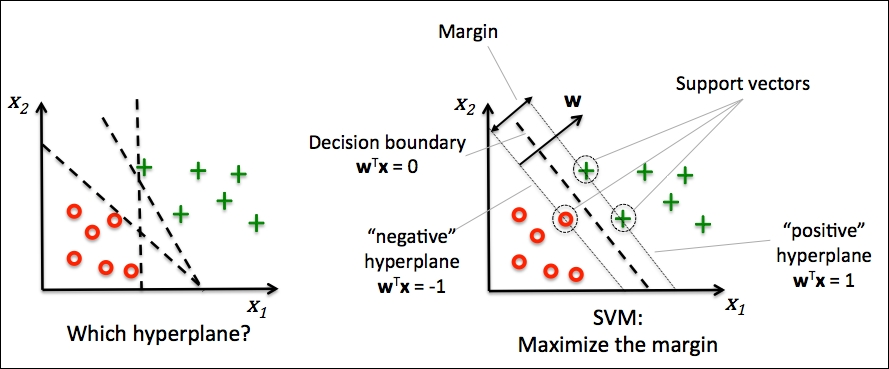
\includegraphics[width=5cm]{svm_maximum_margin_support_vectors.jpg}
\caption*{\raggedright \tiny Maximum Margin Classifier and Support Vectors in SVM}
\end{subfigure}
\begin{subfigure}[b]{.25\textwidth}
\raggedright
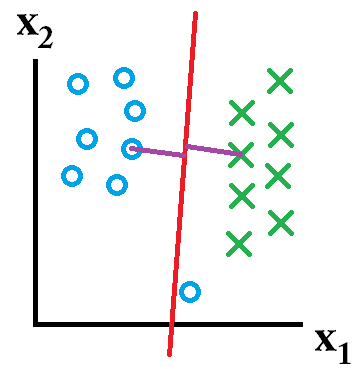
\includegraphics[width=2.0cm]{svm_outlier_cr.png}
\caption*{\raggedleft \tiny Outlier ignored in general SVM.}
\end{subfigure}
\end{figure}
\end{itemize}
\vfill{}
\begin{itemize} 
\fontsize{7}{8.4}\selectfont
\item Linearly Separable Dataset $\rightarrow$ Simple
\item Non-Linearly Separable Dataset $\rightarrow$ Not so simple (kernel trick used)

\begin{figure}
\begin{subfigure}[b]{.4\textwidth}
\centering
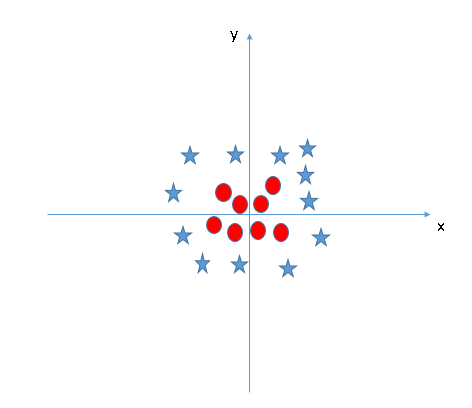
\includegraphics[width=2.5cm]{svm_non_linear_new.png}
\caption*{\centering \tiny Non-linearly separable data}
\end{subfigure}
\begin{subfigure}[b]{.5\textwidth}
\centering
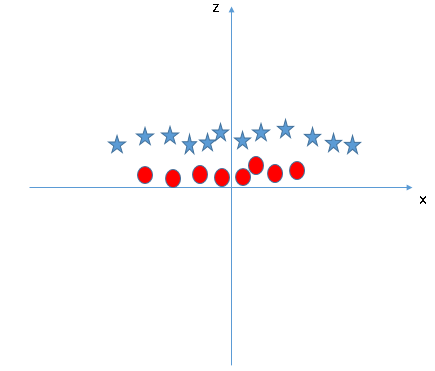
\includegraphics[width=1.7cm]{svm_non_linear_z_axis.png}
\caption*{\centering \tiny Mapping into higher dimension (adding z-axis\linebreak component) Z = \(x^2\) + \(y^2\)}
\end{subfigure}
\end{figure}
\item SVM does not need the actual vectors to work on it, it can do it only with the dot products between them.
This dot product is called a kernel function.
\begin{figure}
\raggedright
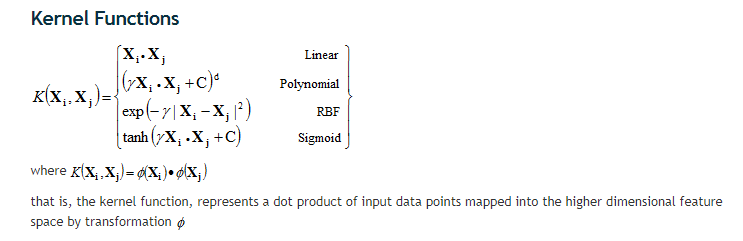
\includegraphics[width=9.5cm]{kernel_functions.png}

\end{figure}
\end{itemize}
\end{frame}



\begin{frame}
\frametitle{\tab \huge Methodology Flow Diagram}
\begin{figure}[!h]
  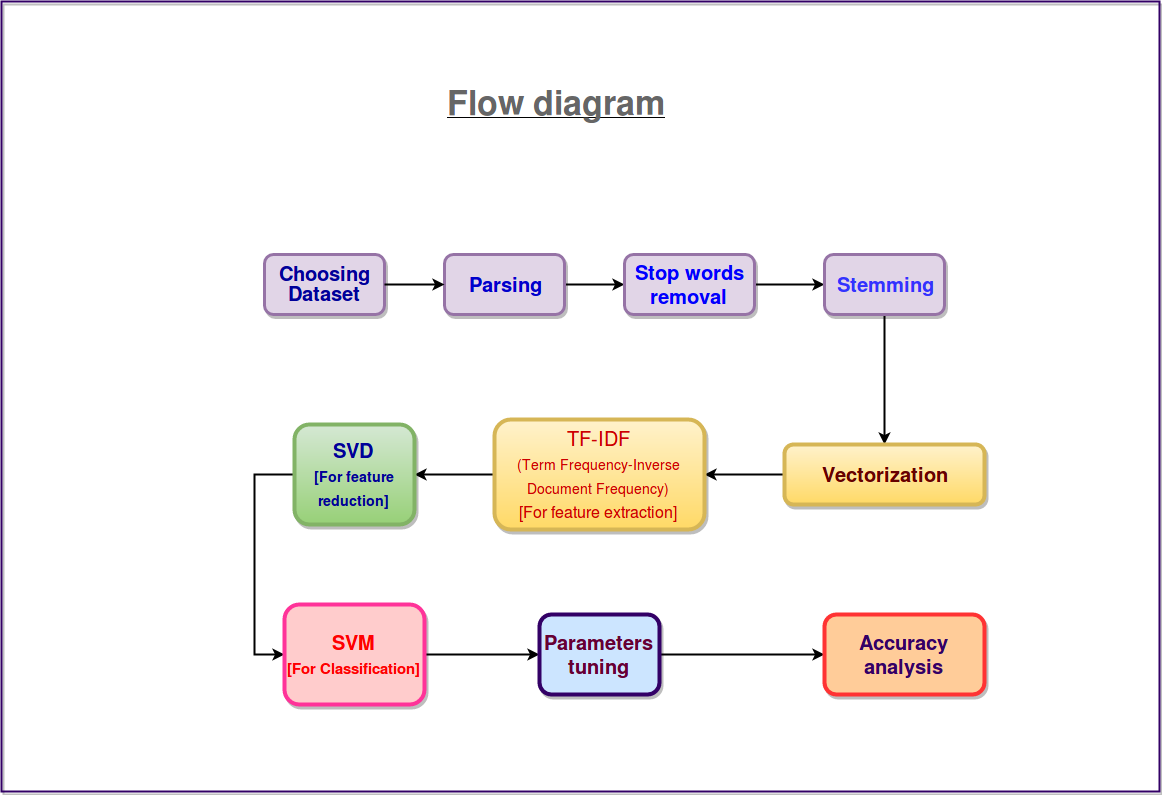
\includegraphics[width=\linewidth]{Flowchart.png}
  \caption{Flow diagram}
  \label{Fig:2}
\end{figure}
\end{frame}

\begin{frame}
\Huge
\centering{
\textbf{\textit{Experiments \\
	\& \\
Observations}}}
\end{frame}

\begin{frame}[t, allowframebreaks]
\frametitle{\tab \tab \tab \Large Experiments and Observations}
\fontsize{8}{9.6}\selectfont
\ \ \ \ \ Change in \textbf{Accuracy} and \textbf{Training time} with change in SVC parameters \textbf{C} and \textbf{gamma}
\linebreak

\begin{vwcol}[widths={6.5,3.0}, sep=.8cm, justify=flush, rule=0pt, indent=1em]
\begin{minipage}{0.7\linewidth}
\tiny
%\raggedleft
\begin{table}[!h]
\label{Fig:}

\begin{tabular}{|p{0.4cm}|p{1.0cm}|p{1.0cm}|p{1.6cm}|p{1.7cm}|}
\hline
\textbf{S.No.} & \textbf{Penalty \t Parameter (C)} & \textbf{Kernel \linebreak Coefficient (gamma)} & \textbf{Training Time (in seconds)} & \textbf{Accuracy \linebreak (\% age)} \\ \hline

1.1            & 1                               & 0                                   & 14.7179185738                       & 53.5163776493              \\ \hline
1.2            & 1                               & 5                                   & 20.2596582446                       & 88.2947976879              \\ \hline
1.3            & 1                               & 10                                  & 49.7798475756                       & 86.8015414258              \\ \hline
2.1            & 10                              & 0                                   & 10.9192837309                       & 80.9730250482              \\ \hline
2.2            & 10                              & 5                                   & 19.5810598891                       & 88.9691714836              \\ \hline
2.3            & 10                              & 10                                  & 50.6595395278                       & 87.2350674374              \\ \hline
3.1            & 100                             & 0                                   & 7.2436635578                        & 86.7052023121              \\ \hline
3.2            & 100                             & 5                                   & 19.2433398237                       & 88.2947976879              \\ \hline
3.3            & 100                             & 10                                  & 50.6608579851                       & 87.1868978805              \\ \hline
4.1            & 1000                            & 0                                   & 6.0687723209                        & 88.1502890173              \\ \hline
4.2            & 1000                            & 5                                   & 19.1799743322                       & 88.2947976879              \\ \hline
4.3            & 1000                            & 10                                  & 50.5428827899                       & 87.1868978805              \\ \hline
5.1            & 10000                           & 0                                   & 6.2777937673                        & 87.6685934489              \\ \hline
5.2            & 10000                           & 5                                   & 19.1768832492                       & 88.2947976879              \\ \hline
5.3            & 10000                           & 10                                  & 50.9507252798                       & 87.1868978805              \\ \hline
6.1            & 100000                          & 0                                   & 7.1739251665                        & 87.5722543353              \\ \hline
6.2            & 100000                          & 5                                   & 19.1878773779                       & 88.2947976879              \\ \hline
6.3            & 100000                          & 10                                  & 50.5921981372                       & 87.1868978805              \\ \hline
7.1            & 1000000                         & 0                                   & 9.7328505405                        & 87.1868978805              \\ \hline
7.2            & 1000000                         & 5                                   & 19.2118927153                       & 88.2947976879              \\ \hline
7.3            & 1000000                         & 10                                  & 50.5413184316                       & 87.1868978805              \\ \hline
\end{tabular}
\end{table}
\end{minipage}
\begin{minipage}{0.3\linewidth}
\textbf{Kernel Function :} \\
Radial Basis Function \\
(rbf) \\

Using different values for the
\textbf{Penalty Parameter ( C )} and
\textbf{Kernel coefficient (gamma )},
the best results we found from
our experiments:\
\begin{itemize}
\item C = 10.0
\item gamma = 5.0
\item Training Time taken =
19.581059889092217
seconds
\item Accuracy on test dataset =
88.969171483622356 \%
\end{itemize}

\end{minipage}
\end{vwcol}

\raggedright
\begin{figure}[!h]
  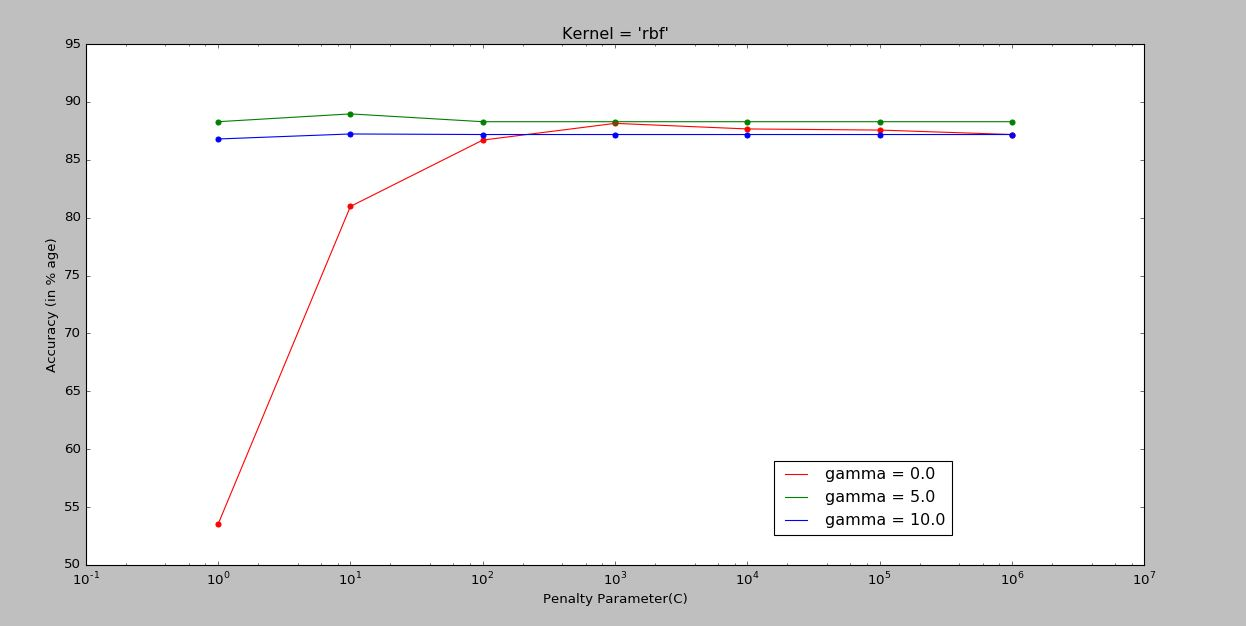
\includegraphics[width=0.8\linewidth]{rbf_all_in_one.JPG}
  \caption*{\tiny \textbf{Accuracy }vs\textbf{ Penalty Parameter (C)} (for \textbf{rbf kernel})}
  \label{fig:}
\end{figure}

\begin{block}
\LARGE Standard deviation = \ \ 12.660401(for gamma = 0.0),\linebreak \tab \tab \tab 0.254889(for gamma = 5.0),\linebreak \tab \tab \tab 0.149765(for gamma = 10.0)
\end{block}
\pagebreak


%\setlength{\columnsep}{10pt}
\fontsize{8}{9.6}\selectfont
\ \ \ \ \ \textbf{Change in Accuracy and Training time with change in SVC parameter C}
\linebreak

\begin{vwcol}[widths={6.5,3.0}, sep=.8cm, justify=flush, rule=0pt, indent=1em]
\begin{minipage}{0.7\linewidth}

\tiny
\begin{table}[!h]
%\raggedleft
\label{Fig:}
\begin{tabular}{|p{0.3cm}|p{0.5cm}|p{1.0cm}|p{1.6cm}|p{1.6cm}|}
\hline
\textbf{S.No.} & \textbf{Kernel} & \textbf{Penalty\linebreak Parameter\linebreak (C)} & \textbf{Training Time (in seconds)} & \textbf{Accuracy \linebreak(\% age)} \\ \hline
1\rule{0pt}{3ex}\linebreak\linebreak              & Linear          & 1                                & 5.7447666912                        & 85.5973025048              \\ \hline
2\rule{0pt}{3ex}\linebreak\linebreak              & Linear          & 10                               & 4.4802451655                        & 88.4393063584              \\ \hline
3\rule{0pt}{3ex}\linebreak\linebreak              & Linear          & 100                              & 4.4675985817                        & 87.9094412331              \\ \hline
4\rule{0pt}{3ex}\linebreak\linebreak              & Linear          & 1000                             & 5.3948755933                        & 87.4759152216              \\ \hline
5\rule{0pt}{3ex}\linebreak\linebreak              & Linear          & 10000                            & 10.4627913232                       & 87.1868978805              \\ \hline
6
\rule{0pt}{3ex}\linebreak\linebreak              & Linear          & 100000                           & 101.2622459789                      & 87.0905587669              \\ \hline
\end{tabular}
\end{table}
%\columnbreak
%\raggedright
\end{minipage}
\begin{minipage}{0.3\linewidth}
\textbf{Kernel Function :} \\
Linear \\

Using different values for the
\textbf{Penalty Parameter ( C )} and
\textbf{Kernel coefficient (gamma )},
the best results we found from
our experiments:\
\begin{itemize}
\item C = 10.0
\item Training Time taken =
4.48024516547855 seconds
\item Accuracy on test dataset =
88.439306358381498 \%
\end{itemize}

\end{minipage}
\end{vwcol}


\begin{figure}[!h]
  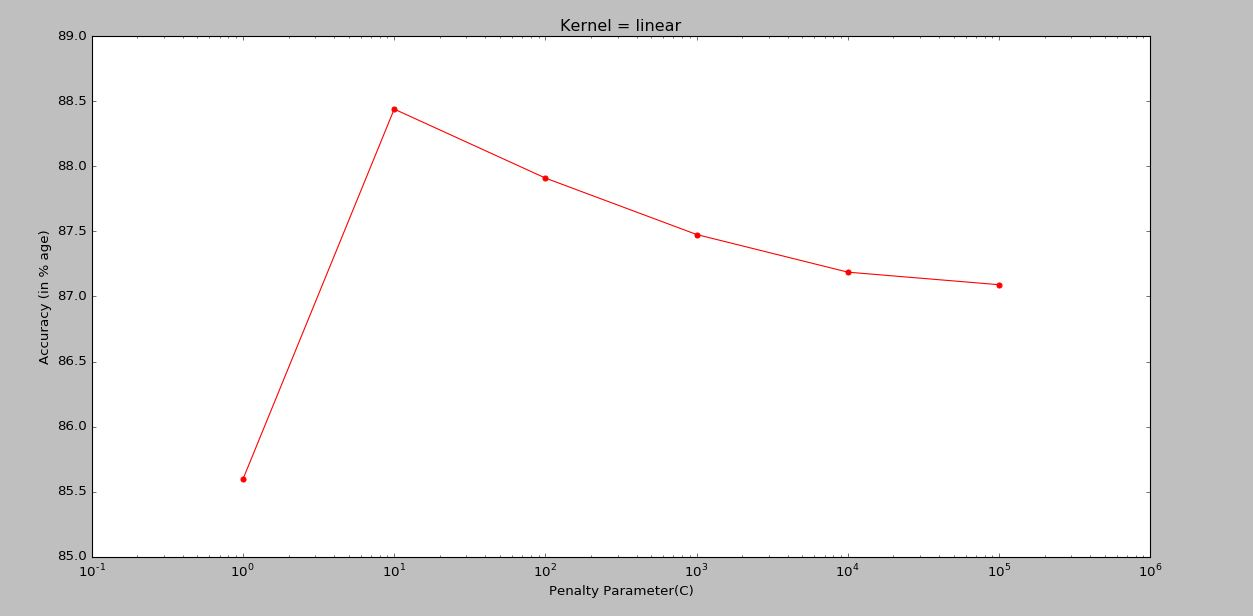
\includegraphics[width=0.8\linewidth]{linear.JPG}
  \caption*{\tiny \textbf{Accuracy }vs\textbf{ Penalty Parameter (C)} (for \textbf{linear kernel} with \textbf{gamma} = 0.0, 5.0 and 10.0))}
  \label{fig:}
\end{figure}
\begin{exampleblock}
\LARGE
Standard deviation = 0.964835
\end{exampleblock}
\pagebreak
\fontsize{8}{9.6}\selectfont
{\textbf{Average Accuracy} and \textbf{Average Training Time} with different random splits of Training and Test}
\linebreak

\begin{vwcol}[widths={6.5,3.0}, sep=.8cm, justify=flush, rule=0pt, indent=1em]
\begin{minipage}{0.7\linewidth}

\tiny
\begin{table}[!h]
%\raggedleft
\label{Fig:}
\fontsize{5}{6}\selectfont
\begin{tabular}{|p{0.3cm}|p{0.4cm}|p{0.6cm}|p{1.0cm}|p{1.0cm}|p{1.1cm}|p{1.0cm}|}
\hline
\textbf{S.No.}             & \textbf{Penalty Parameter (C)} & \textbf{Kernel Coefficient (gamma)} & \textbf{Average Training \linebreak Time \linebreak (in seconds)} & \textbf{Average \linebreak Accuracy \linebreak (\% age)} & \textbf{Minimum \linebreak Accuracy \linebreak (\% age)} & \textbf{Maximum \linebreak Accuracy \linebreak (\% age)} \\ \hline
1\rule{0pt}{3ex}\linebreak\linebreak             & 10                              & 5                                   & 19.5975905119                               & 87.591522158                       & 86.8497109827                     & 88.1984585742                     \\ \hline
2\rule{0pt}{3ex}\linebreak\linebreak              & 1                               & 5                                   & 19.8280292122                               & 88.2369942197                      & 88.0539499037                     & 88.3429672447                     \\ \hline
3\rule{0pt}{3ex}\linebreak\linebreak              & 100                             & 5                                   & 19.1036437403                               & 86.5317919075                      & 85.9344894027                     & 86.7052023121                     \\ \hline
4\rule{0pt}{3ex}\linebreak\linebreak              & 1000                            & 5                                   & 18.7571186214                               & 87.9768786127                      & 87.1868978805                     & 88.1984585742                     \\ \hline
5\rule{0pt}{3ex}\linebreak\linebreak              & 10000                           & 5                                   & 20.2823468282                               & 88.7379576108                      & 87.8612716763                     & 89.2581888247                     \\ \hline
\end{tabular}
\end{table}
%\columnbreak
%\raggedright
\end{minipage}
\begin{minipage}{0.3\linewidth}
\textbf{Kernel Function :} \\
Radial Basis Function (rbf) \\

Using different random splits of training and test datasets for fixed value of SVC parameters, the best results we found are : 
\begin{itemize}
\item C = 10000.0
\item gamma = 5.0
\item Average Training Time
taken =
20.28234682823986
\item Average Accuracy on test
dataset =
88.737957610789986 \%
\end{itemize}

\end{minipage}
\end{vwcol}


\begin{figure}[!h]
  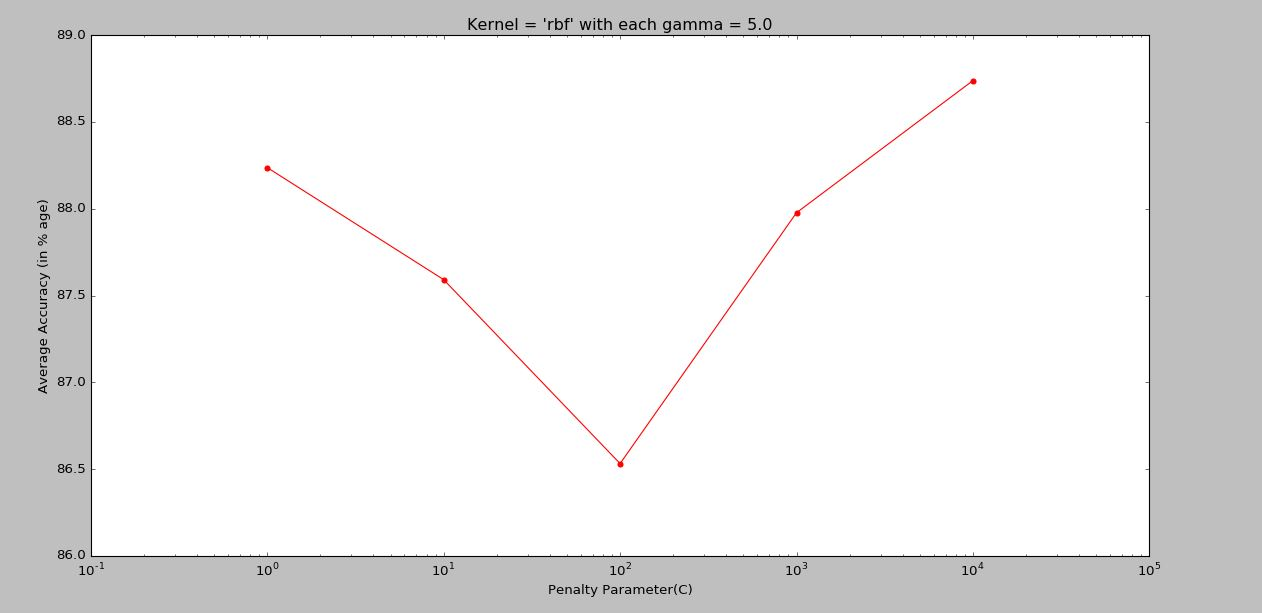
\includegraphics[width=0.8\linewidth]{kuchbhi.jpg}
  \caption*{\tiny \textbf{Accuracy }vs\textbf{ Penalty Parameter (C)} (for \textbf{rbf kernel} with different splits of training and test data)}
  \label{fig:}
\end{figure}
\begin{block}
\LARGE Standard deviation = 0.829563
\end{block}
\pagebreak

\fontsize{8}{9.6}\selectfont
\textbf{Average Accuracy} and \textbf{Average Training time} with different
random splits of training and test
\linebreak


\begin{vwcol}[widths={6.5,3.0}, sep=.8cm, justify=flush, rule=0pt, indent=1em]
\begin{minipage}{0.7\linewidth}
\tiny
\begin{table}[!h]
%\raggedleft
\label{Fig:}
\fontsize{5}{6}\selectfont
\begin{tabular}{|p{0.3cm}|p{0.6cm}|p{1.1cm}|p{1.1cm}|p{1.1cm}|p{1.1cm}|}
\hline
\textbf{S.No.} & \textbf{Penalty\linebreak Parameter\linebreak (C)} & \textbf{Average Training\linebreak Time\linebreak(in seconds)} & \textbf{Average Accuracy\linebreak (\% age)} & \textbf{Minimum Accuracy\linebreak (\% age)} & \textbf{Maximum Accuracy \linebreak (\% age)} \\ \hline
1\rule{0pt}{3ex}\linebreak\linebreak              & 10                              & 26.4541190135                               & 86.3102119461                      & 85.3082851638                     & 87.6685934489                     \\ \hline
2\rule{0pt}{3ex}\linebreak\linebreak              & 100                             & 19.0949781875                               & 87.3603082852                      & 86.6570327553                     & 88.8728323699                     \\ \hline
3\rule{0pt}{3ex}\linebreak\linebreak              & 1000                            & 26.5995590032                               & 85.4624277457                      & 84.4894026975                     & 86.8978805395                     \\ \hline
4\rule{0pt}{3ex}\linebreak\linebreak              & 10000                           & 19.1290173923                               & 87.2832369942                      & 86.4161849711                     & 88.5356454721                     \\ \hline
5\rule{0pt}{3ex}\linebreak\linebreak              & 100000                          & 22.8623470763                               & 88.1695568401                      & 87.4759152216                     & 89.0655105973                     \\ \hline
\end{tabular}
\end{table}
%\columnbreak
%\raggedright
\end{minipage}
\begin{minipage}{0.3\linewidth}
\textbf{Kernel Function :} \\
Linear \\

Using different random splits
of training and test datasets
for fixed value of svc
parameters the best results
we found are:
\begin{itemize}
\item C = 100000.0
\item Average Training Time
taken =
22.862347076279367
seconds
\item Average Accuracy on test
dataset =
88.169556840077068 \%
\end{itemize}

\end{minipage}
\end{vwcol}


\begin{figure}[!h]
  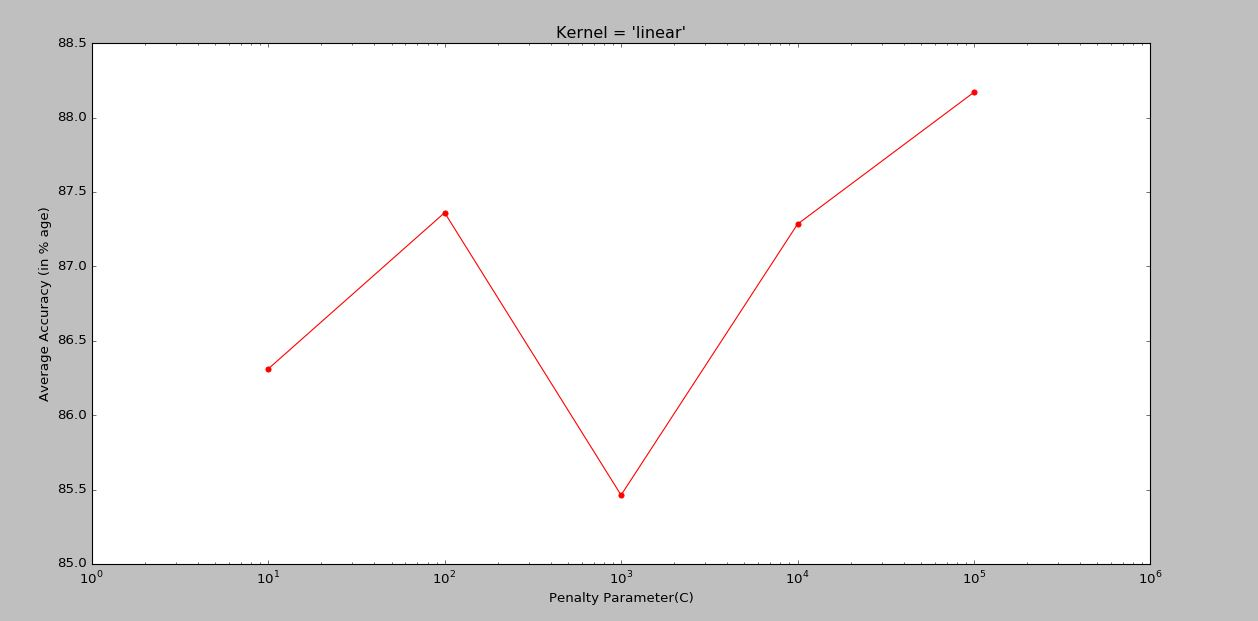
\includegraphics[width=0.8\linewidth]{linear_for_different_randomstates.JPG}
  \caption*{\tiny \textbf{Accuracy }vs\textbf{ Penalty Parameter (C)} (for \textbf{linear kernel} with different splits of training and test data)}
  \label{fig:}
\end{figure}
\begin{block}
\LARGE Standard deviation = 1.046843
\end{block}



\end{frame}

\begin{frame}
\frametitle{\tab \tab \tab \huge Generic Text Classifier}
After training and testing on \enquote{Reuters Dataset} we created Generic Text Classification model. \\
We tested our text classification model on various small datasets.\linebreak \linebreak
The average accuracy obtained for various datasets:-\\
\begin{enumerate}
\item Amazon review = 75.74\% ( data size = 1000 , kernel = linear )\\
\item IMDb review = 73.83\% ( data size = 1000 , kernel = linear )\\
\item Yelp review = 77.03\% ( data size = 1000 , kernel = linear )\\
\item Spam Detection = 96.34\% ( best we obtained till now , data size = 5574 ,
kernel = linear )\\
\item News Headline = 90.71\% ( data size = 5977 , kernel = rbf )\\
\end{enumerate}
\end {frame}

\begin{frame}
\frametitle{\quad \huge Amazon Online Review Binary-Classifier}

For amazon review dataset we trained it and tested it on the splitted portion,\\
Once this part was over, we modified our model and made it online , \linebreak \linebreak
\begin{enumerate}
\item now it takes review from user.\\
\item extracts and reduces the features complete dataset (original+user input) using SVD.\\
\item training is done only for our previous dataset. \\
\item then the review is accordingly classified \\
\item the user entered review is added to our dataset after classification \linebreak \linebreak
\end{enumerate}
This added data helps us to improve accuracy if similar input is given again

\end{frame}

\begin{frame}
\frametitle{\tab \tab \tab \tab \huge Future Work}
\begin{itemize}
\item Till now we have trained and tested our model on the same dataset. So there is a high chance of getting good accuracy. \linebreak
\item Our future challenge would be to train our model on one dataset and using its extracted features, try to classify(test) different but related dataset. \linebreak
\item As suggested by our instructor, we can solve this problem through Transfer Learning.
\end{itemize}
\end {frame}

\begin{frame}
\frametitle{\tab \tab \tab \tab \huge Transfer Learning}
\begin{itemize}
\item Transfer learning is an emerging field in Machine Learning.
\item It involves using knowledge extracted while solving one problem to apply it to a related but different problem.
\item For instance, we could train our model on X news agency\textquotesingle s(say FOX News) dataset and test on Y news agency\textquotesingle s(say ABC news) dataset and analyse the features which lead to anomalous results.
\item We could then adjust our model to these features, in order to develop a generic model which gives accurate results for most of the datasets in this domain(News).
\item For transfer learning to work effectively we need to recognise and include those features in main features list which for effective knowledge extension.
\end{itemize}
\end {frame}

\begin{frame}
\frametitle{\tab \tab \tab \quad \quad \quad \huge Challenges}
\begin{itemize}
\item During concluding part of our project,we worked on applying transfer learning in our model. We trained our model on News Articles Data(obtained from web scraping ) dataset and tried to test it on another dataset which contains News Headlines only but we faced various challenges. \\
\item For instance,when we trained our model with a larger dataset with 5000 features and test on a smaller dataset (say with 100 features,) our objective was to extract features from the bigger dataset which are common in both the datasets.Finally ,scale features of both the datasets on a common scale. \\
\item We tried to use SVD for feature reduction but it didn\textquotesingle t yield required results as applying SVD individually gives different scales for the two sets of
features. The basic requirement for a effective transfer learning is that no. of
features in training dataset should be equivalent to features in testing dataset.\\
\item We look forward to overcoming this problem and work on new approach to implement transfer learning.
\end{itemize}
\end {frame}


\begin{frame}[t, allowframebreaks]
\frametitle{\tab \tab \tab \tab \huge Softwares Used}
\textbf{IDE used :}
\begin{itemize}
\item Spyder 3 (Scientific PYthon Development EnviRonment)
\end{itemize}
\textbf{Language used :}
\begin{itemize}
\item Python 3.5
\end{itemize}
\textbf{Libraries Used :}
\begin{itemize}
\item \textbf{pandas (Python Data Analysis Library)} for inputting the Dataset (.tsv file).

\item The module \textbf{pyplot} of matplotlib library is used for graph plotting
re library for the usage of Regular Expressions for text cleaning.

\item Stopwords list from the \lq \textbf{corpus}\rq \ package of \textbf{nltk} (Natural Language Processing Toolkit) data package.

\item \textbf{PorterStemmer} algorithm from the package nltk.stem.porter for stemming of words.

\item \textbf{CountVectorizer} class from sklearn.feature\_extraction.text submodule for building the matrix (sparse) of word counts from text documents.

\item \textbf{TfidfTransformer} class from sklearn.feature\_extraction.text submodule to convert the count matrix (sparse) to a matrix of TF\_IDF features.

\item \textbf{TruncatedSVD} class from sklearn.decomposition module for dimensionality reduction of the feature space.

\item \textbf{train\_test\_split} function from sklearn.cross\_validation module for splitting the whole Dataset into random train and test sunsets.

\item \textbf{SVC} class from \textbf{sklearn.svm} module for classification of the test set.
\end{itemize}
\end{frame}

\tiny
\begin{frame}[t,allowframebreaks]
\frametitle {\tab \tab \tab \tab \huge References}
\bibliographystyle{plain}
\bibliography{references.bib}
\end{frame}

%------------------------------------------------
\end{document}